% В этом файле следует писать текст работы, разбивая его на
% разделы (section), подразделы (subsection) и, если нужно,
% главы (chapter).

% Предварительно следует указать необходимую информацию
% в файле SETUP.tex

%% В этот файл не предполагается вносить изменения

% В этом файле следует указать информацию о себе
% и выполняемой работе.

\documentclass [fontsize=14pt, paper=a4, pagesize, DIV=calc]%
{scrartcl}
% ВНИМАНИЕ! Для использования глав поменять
% scrartcl на scrreprt

% Здесь ничего не менять
\usepackage [T2A] {fontenc}   % Кириллица в PDF файле
\usepackage [utf8] {inputenc} % Кодировка текста: utf-8
\usepackage [russian] {babel} % Переносы, лигатуры

%%%%%%%%%%%%%%%%%%%%%%%%%%%%%%%%%%%%%%%%%%%%%%%%%%%%%%%%%%%%%%%%%%%%%%%%
% Создание макроса управления элементами, специфичными
% для вида работы (курс., бак., маг.)
% Здесь ничего не менять:
\usepackage{ifthen}
\newcounter{worktype}
\newcommand{\typeOfWork}[1]
{
	\setcounter{worktype}{#1}
}

% ВНИМАНИЕ!
% Укажите тип работы: 0 - курсовая, 1 - бак., 2 - маг.,
% 3 - бакалаврская с главами.
\typeOfWork{1}
% Считается, что курсовая и бак. бьются на разделы (section) и
% подразделы (subsection), а маг. — на главы (chapter), разделы и
%  подразделы. Если хочется,
% чтобы бак. была с главами (например, если она большая),
% надо выбрать опцию 3.

% Если при выборе 2 или 3 вы забудете поменять класс
% документа на scrreprt (см. выше, в самом начале),
% то получите ошибку:
% ./aux/appearance.tex:52: Package scrbase Error: unknown option ` chapterprefix=

%%%%%%%%%%%%%%%%%%%%%%%%%%%%%%%%%%%%%%%%%%%%%%%%%%%%%%%%%%%%%%%%%%%%%%%%
% Информация об авторе и работе для титульной страницы

\usepackage {titling}

% Имя автора в именительном падеже (для маг.)
\newcommand {\me}{%
М.\,И.~Глухова
}

% Имя автора в родительном падеже (для курсовой и бак.)
\newcommand {\byme}{%
М.\,И.~Глуховой%
}

% Научный руководитель
\newcommand{\supervisor}%
{профессор, д.ф.-м.н. В. С. Пилиди}

% идентифицируем пол (только для курсовой и бак.)
\newcommand{\bystudent}{
студентки
}

% Год публикации
\date{2015}

% Название работы
\title{Программная реализация алгоритмов поиска \\аналитических кривых на изображении}

% Кафедра
%

\newcommand {\direction} {%
Направление подготовки\\02.\ifthenelse{\value{worktype} = 2}{04}{03}.02 ---
Фундаментальная информатика\\и информационные технологии%
}

%%%%%%%%%%%%%%%%%%%%%%%%%%%%%%%%%%%%%%%%%%%%%%%%%%%%%%%%%%%%%%%%%%%%%%%%
% Другие настраиваемые элементы текста

% Листинги с исходным кодом программ: укажите язык программирования
\usepackage{listings}
\lstset{
    language=[ISO]C++,%  Язык указать здесь
    basicstyle=\small\ttfamily,
    breaklines=true,%
    showstringspaces=false%
    inputencoding=utf8x%
}
% полный список языков, поддерживаемых данным пакетом, есть,
% например, здесь (стр. 13):
% ftp://ftp.tex.ac.uk/tex-archive/macros/latex/contrib/listings/listings.pdf

% Нумерация списков: можно при необходимести
% изменять вид нумерации (например, добавлять правую скобку).
% По умолчанию буду списки вида:
% 1.
% 2.
% Изменять вид нумерации можно в начале нумерации:
% \begin{enumerate}[1)] (В квадратных скобках указан желаемый вид)
\usepackage[shortlabels]{enumitem}
                    \setlist[enumerate, 1]{1.}

% Гиперссылки: настройте внешний вид ссылок
\usepackage%
[pdftex,unicode,pdfborder=0,draft=false,%backref=page,
    hidelinks, % убрать, если хочется видеть ссылки: это
               % удобно в PDF файле, но не должно появиться на печати
    bookmarks=true,bookmarksnumbered=false,bookmarksopen=false]%
{hyperref}


\usepackage {amsmath}      % Больше математики
\usepackage {amssymb}
\usepackage {textcase}     % Преобразование к верхнему регистру
\usepackage {indentfirst}  % Красная строка первого абзаца в разделе

\usepackage {fancyvrb}     % Листинги: определяем своё окружение Verb
\DefineVerbatimEnvironment% с уменьшенным шрифтом
	{Verb}{Verbatim}
	{fontsize=\small}

% Вставка рисунков
\usepackage {graphicx}

% Графики
\usepackage{pgfplots}

% Общее оформление
% ----------------------------------------------------------------
% Настройка внешнего вида

%%% Шрифты

% если закомментировать всё — консервативная гарнитура Computer Modern
\usepackage{paratype} % профессиональные свободные шрифты
%\usepackage {droid}  % неплохие свободные шрифты от Google
%\usepackage{mathptmx}
%\usepackage {mmasym}
%\usepackage {psfonts}
%\usepackage{lmodern}
%var1: lh additions for bold concrete fonts
%\usepackage{lh-t2axccr}
%var2: the package below could be covered with fd-files
%\usepackage{lh-t2accr}
%\usepackage {pscyr}

% Геометрия текста

\usepackage{setspace}       % Межстрочный интервал
\onehalfspacing

\newlength\MyIndent
\setlength\MyIndent{1.25cm}
\setlength{\parindent}{\MyIndent} % Абзацный отступ
\frenchspacing            % Отключение лишних отступов после точек
\KOMAoptions{%
    DIV=calc,         % Пересчёт геометрии
    numbers=endperiod % точки после номеров разделов
}

                            % Консервативный вариант:
%\usepackage                % ручное задание геометрии
%[%                         % (не рекомендуется в проф. типографии)
%  margin = 2.5cm,
  %includefoot,
  %footskip = 1cm
%] %
%  {geometry}

%%% Заголовки

\ifthenelse{\equal{\theworktype}{2}}{%
\KOMAoptions{%
    numbers=endperiod,% точки после номеров разделов
    headings=normal,   % размеры заголовков поменьше стандартных
    chapterprefix=true,% Печатать слово Глава в магистерской
    appendixprefix=true% Печатать слово Приложение
}
}

% шрифт для оформления глав и названия содержания
\newcommand{\SuperFont}{\Large\sffamily\bfseries}

% Заголовок главы
\ifthenelse{\value{worktype} > 1}{%
\renewcommand{\SuperFont}{\Large\normalfont\sffamily}
\newcommand{\CentSuperFont}{\centering\SuperFont}
\usepackage{fncychap}
\ChNameVar{\SuperFont}
\ChNumVar{\CentSuperFont}
\ChTitleVar{\CentSuperFont}
\ChNameUpperCase
\ChTitleUpperCase
}

% Заголовок (под)раздела с абзацного отступа
\addtokomafont{sectioning}{\hspace{\MyIndent}}

\renewcommand*{\captionformat}{~---~}
\renewcommand*{\figureformat}{Рисунок~\thefigure}

% Плавающие листинги
\usepackage{float}
\floatstyle{ruled}
\floatname{ListingEnv}{Листинг}
\newfloat{ListingEnv}{htbp}{lol}[section]

% точка после номера листинга
\makeatletter
\renewcommand\floatc@ruled[2]{{\@fs@cfont #1.} #2\par}
\makeatother


%%% Оглавление
\usepackage{tocloft}

% шрифт и положение заголовка
\ifthenelse{\value{worktype} > 1}{%
\renewcommand{\cfttoctitlefont}{\hfil\SuperFont\MakeUppercase}
}{
\renewcommand{\cfttoctitlefont}{\hfil\SuperFont}
}

% слово Глава
\usepackage{calc}
\ifthenelse{\value{worktype} > 1}{%
\renewcommand{\cftchappresnum}{Глава }
\addtolength{\cftchapnumwidth}{\widthof{Глава }}
}

% Очищаем оформление названий старших элементов в оглавлении
\ifthenelse{\value{worktype} > 1}{%
\renewcommand{\cftchapfont}{}
\renewcommand{\cftchappagefont}{}
}{
\renewcommand{\cftsecfont}{}
\renewcommand{\cftsecpagefont}{}
}

% Точки после верхних элементов оглавления
\renewcommand{\cftsecdotsep}{\cftdotsep}
%\newcommand{\cftchapdotsep}{\cftdotsep}

\ifthenelse{\value{worktype} > 1}{%
    \renewcommand{\cftchapaftersnum}{.}
}{
\renewcommand{\cftsecaftersnum}{.}
\renewcommand{\cftsubsecaftersnum}{.}
}
%%% Списки (enumitem)

\usepackage {enumitem}      % Списки с настройкой отступов
\setlist %
{ %
  leftmargin = \parindent, itemsep=.5ex, topsep=.4ex
} %

% По ГОСТу нумерация должны быть буквами: а, б...
%\makeatletter
%    \AddEnumerateCounter{\asbuk}{\@asbuk}{м)}
%\makeatother
%\renewcommand{\labelenumi}{\asbuk{enumi})}
%\renewcommand{\labelenumii}{\arabic{enumii})}

%%% Таблицы: выбрать более подходящие

\usepackage{booktabs} % считаются наиболее профессионально выполненными
%\usepackage{ltablex}
%\newcolumntype {L} {>{---}l}

%%% Библиография

\usepackage{csquotes}        % Оформление списка литературы
\usepackage[
  backend=biber,
  hyperref=auto,
  sorting=none, % сортировка в порядке встречаемости ссылок
  language=auto,
  citestyle=gost-numeric,
  bibstyle=gost-numeric
]{biblatex}
\addbibresource{biblio.bib} % Файл с лит.источниками

% Настройка величины отступа в списке
\ifthenelse{\value{worktype} < 2}{%
\defbibenvironment{bibliography}
  {\list
     {\printtext[labelnumberwidth]{%
    \printfield{prefixnumber}%
    \printfield{labelnumber}}}
     {\setlength{\labelwidth}{\labelnumberwidth}%
      \setlength{\leftmargin}{\labelwidth}%
      \setlength{\labelsep}{\dimexpr\MyIndent-\labelwidth\relax}% <----- default is \biblabelsep
      \addtolength{\leftmargin}{\labelsep}%
      \setlength{\itemsep}{\bibitemsep}%
      \setlength{\parsep}{\bibparsep}}%
      \renewcommand*{\makelabel}[1]{\hss##1}}
  {\endlist}
  {\item}
}{}

% ----------------------------------------------------------------
% Настройка переносов и разрывов страниц

\binoppenalty = 10000      % Запрет переносов строк в формулах
\relpenalty = 10000        %

\sloppy                    % Не выходить за границы бокса
%\tolerance = 400          % или более точно
\clubpenalty = 10000       % Запрет разрывов страниц после первой
\widowpenalty = 10000      % и перед предпоследней строкой абзаца

% ----------------------------


% Стили для окружений типа Определение, Теорема...
% Оформление теорем (ntheorem)

\usepackage [thmmarks, amsmath] {ntheorem}
\theorempreskipamount 0.6cm

\theoremstyle {plain} %
\theoremheaderfont {\normalfont \bfseries} %
\theorembodyfont {\slshape} %
\theoremsymbol {\ensuremath {_\Box}} %
\theoremseparator {:} %
\newtheorem {mystatement} {Утверждение} [section] %
\newtheorem {mylemma} {Лемма} [section] %
\newtheorem {mycorollary} {Следствие} [section] %

\theoremstyle {nonumberplain} %
\theoremseparator {.} %
\theoremsymbol {\ensuremath {_\diamondsuit}} %
\newtheorem {mydefinition} {Определение} %

\theoremstyle {plain} %
\theoremheaderfont {\normalfont \bfseries} 
\theorembodyfont {\normalfont} 
%\theoremsymbol {\ensuremath {_\Box}} %
\theoremseparator {.} %
\newtheorem {mytask} {Задача} [section]%
\renewcommand{\themytask}{\arabic{mytask}}

\theoremheaderfont {\scshape} %
\theorembodyfont {\upshape} %
\theoremstyle {nonumberplain} %
\theoremseparator {} %
\theoremsymbol {\rule {1ex} {1ex}} %
\newtheorem {myproof} {Доказательство} %

\theorembodyfont {\upshape} %
%\theoremindent 0.5cm
\theoremstyle {nonumberbreak} \theoremseparator {\\} %
\theoremsymbol {\ensuremath {\ast}} %
\newtheorem {myexample} {Пример} %
\newtheorem {myexamples} {Примеры} %

\theoremheaderfont {\itshape} %
\theorembodyfont {\upshape} %
\theoremstyle {nonumberplain} %
\theoremseparator {:} %
\theoremsymbol {\ensuremath {_\triangle}} %
\newtheorem {myremark} {Замечание} %
\theoremstyle {nonumberbreak} %
\newtheorem {myremarks} {Замечания} %

% Титульный лист
% Макросы настройки титульной страницы
% В этот файл не предполагается вносить изменения

%\usepackage {showframe}

% Вертикальные отступы на титульной странице
\newcommand{\vgap}{\vspace{16pt}}

% Помещение города и даты в нижний колонтитул
\usepackage{scrlayer}
\DeclareNewLayer[
  foot,
  foreground,
  contents={%
    \raisebox{\dp\strutbox}[\layerheight][0pt]{%
      \parbox[b]{\layerwidth}{\centering Ростов-на-Дону\\ \thedate%
       \\\mbox{}
       }}%
  }
]{titlepage.foot.fg}
\DeclareNewPageStyleByLayers{titlepage}{titlepage.foot.fg}


\AtBeginDocument %
{ %
  %
  \begin{titlepage}
  %
    \thispagestyle{titlepage}

    {\centering
    %
    \MakeTextUppercase {МИНИСТЕРСТВО ОБРАЗОВАНИЯ И НАУКИ РФ}

    \vgap

    Федеральное государственное автономное образовательное\\
    учреждение высшего образования\\
    \MakeTextUppercase {Южный федеральный университет}

    \vgap

	Институт математики, механики и компьютерных наук
    имени~И.\,И.\,Воровича

    \vgap

    \direction

    \vspace* {\fill}

    \ifthenelse{\value{worktype} = 2}{%
    \me

    \vgap}{}

    \MakeTextUppercase{\thetitle}

    \ifthenelse{\value{worktype} = 2}{%
     \vgap

    Магистерская диссертация}{}
    \ifthenelse{\value{worktype} = 0}{
     \vgap

    Курсовая работа
    }{}%
    \ifthenelse{\value{worktype} = 1 \OR \value{worktype} = 3}{
     \vgap

    Выпускная квалификационная работа\\
    на степень бакалавра
    }{}%

    \vspace {\fill}

    \begin{flushright}
    \ifthenelse{\value{worktype} = 1 \OR \value{worktype} = 0}{
      \bystudent \ifthenelse{\value{worktype} = 0}{3}{4}\ курса\\
      \byme
    }{}

    \vgap

Научный руководитель:\\
    \supervisor\\
    \ifthenelse{\value{worktype} = 2}{%
    Рецензент:\\
    ученая степень, ученое звание [, должность]
    И. О. Фамилия
    }{}
	\end{flushright}
\ifthenelse{\value{worktype} = 0}{
\vspace{\fill}
        \begin{flushleft}
          \begin{tabular}{cc}
            \underline{\hspace{4cm}}&\underline{\hspace{5cm}}\\
            {\small оценка (рейтинг)} & {\small  подпись руководителя}\\
          \end{tabular}
          \\[1cm]
%          Утверждаю:\\руководитель направления ФИИТ \underline{\hspace{4cm}}
%В.\,С.\,Пилиди
        \end{flushleft}
}{}
\ifthenelse{\value{worktype} = 1 \OR \value{worktype} = 3}{
\vspace{\fill}
        \begin{flushleft}
Допущено к защите:\\руководитель направления ФИИТ
\underline{\hspace{4cm}}
В.\,С.\,Пилиди
        \end{flushleft}
}{}


  	\vspace {\fill}

  %Ростов-на-Дону

    %\thedate

  }\end{titlepage}
  %
  %
  %\tableofcontents
  %
  \clearpage
} %


% Команды для использования в тексте работы
% макросы для начала введения и заключения
\newcommand{\Intro}{\addsec{Введение}}
\ifthenelse{\value{worktype} > 1}{%
    \renewcommand{\Intro}{\addchap{Введение}}%
}

\newcommand{\Conc}{\addsec{Заключение}}
\ifthenelse{\value{worktype} > 1}{%
    \renewcommand{\Conc}{\addchap{Заключение}}%
}

% и еще постановку задачи
\newcommand{\Task}{\addsec{Постановка задачи}}
\ifthenelse{\value{worktype} > 1}{%
    \renewcommand{\Task}{\addchap{Постановка задачи}}%
}

% Правильные значки для нестрогих неравенств и пустого множества
\renewcommand {\le} {\leqslant}
\renewcommand {\ge} {\geqslant}
\renewcommand {\emptyset} {\varnothing}

% N ажурное: натуральные числа
\newcommand {\N} {\ensuremath{\mathbb N}}

% значок С++ — используйте команду \cpp
\newcommand{\cpp}{%
C\nolinebreak\hspace{-.05em}%
\raisebox{.2ex}{+}\nolinebreak\hspace{-.10em}%
\raisebox{.2ex}{+}%
}

% Неразрывный дефис, который допускает перенос внутри слов,
% типа жёлто-синий: нужно писать жёлто"/синий.
\makeatletter
    \defineshorthand[russian]{"/}{\mbox{-}\bbl@allowhyphens}
\makeatother


\endinput

% Конец файла

\begin{document}

\Task
\begin{enumerate}
  \item
Разработать алгоритм для поиска эллипсов на изображении.
  \item
Реализовать разработанный алгоритм.
  \item
Протестировать работу полученной программы.
\end{enumerate}
\clearpage


\tableofcontents
\clearpage

\Intro
Поиск аналитических кривых на изображении является важной задачей компьютерного зрения и смежных областей. Выделение областей, заданных такими кривыми, помогает в распознавании более сложных фигур.

Преобразование Хафа - алгоритм, часто использующийся для поиска объектов, принадлежащих классу заранее заданных фигур. 
Поиск объектов проходит при помощи процедуры голосования - каждая точка контура "голосует" за объект с теми параметрами, которым она может принадлежать. 
Изначально алгоритм использовался для поиска прямых, затем он был обобщен для поиска линий более общего вида~\autocite{Duda}.
Преобразование Хафа является распространенным инструментом для поиска объектов на изображении, но становится все более затратным по времени и памяти с увеличением количества параметров в уравнении кривой.

Одним из способов уменьшить затраты по времени и памяти является иерархический подход, в котором поиск производится на изображении небольшого размера, а затем полученные параметры уточняются. 
Другой модификацией алгоритма является снижение затрат по памяти за счет использования некоторых соотношений между параметрами эллипса.
В настоящей работе эти два подхода соединены для достижения наибольшей экономии по времени и памяти.

Предполагается, что дано изображение достаточно большого размера, на котором требуется найти один или несколько эллипсов, определив их параметры: 
координаты центра \((x_0, y_0)\), длины большой и малой полуосей \(a\) и \(b\), а также поворот. Предполагается, что все эллипсы, если они есть, лежат 
полностью внутри изображения. При этом не обязательно, чтобы эллипс был представлен целиком - его контур может прерываться или перекрываться. 
Однако требуется, чтобы краевые точки большой оси эллипса на изображении были представлены, так как именно по ним ведется поиск.  

Алгоритм работает как для изображений в оттенках серого, так и для цветных изображений.

\section{Исследование предметной области}
Существуют различные подходы к проблеме поиска эллипсов на изображении.  Большинство из них являются модификациями алгоритма Хафа, 
но испльзовались и такие подходы, как группировка контуров и генетические алгоритмы.

Если использовать для поиска эллипсов ту же стратегию, что и для прямых и окружностей, алгоритм будет описываться приблизительно так (считаем, что изображение имеет размер $N \times N$):
\begin{enumerate}
\item Для каждого ненулевого пиксела изображения (максимум $N \times N$ вариантов):
\item Выбирается первый фокус (в предположении, что фокусы расположены на изображении, а не за его пределами - $N \times N$ вариантов).
\item Выбирается второй фокус ($N \times N$ вариантов).
\item Вычисляется поворот и остальные параметры эллипса.
\item В аккумуляторном массиве значение, соответствующее найденным параметрам (центр, поворот, два радиуса)
\end{enumerate}

Алгоритм в таком виде будет иметь временную сложность \(O(N^6)\), а также потребует хранения 5-мерного аккумуляторного массива. По этим причинам на практике такая реализация неприменима.
Чтобы использовать преобразование Хафа для поиска эллипсов, требуется модифицировать его, уменьшив время работы и требуемую память.

Один из первых алгоритмов, обобщающих преобразование Хафа на аналитические кривые, был предложен в работе~\autocite{Ballard}, 
однако для него требуется заранее знать отклонения искомого объекта (сжатие, поворот) относительно канонической формы, либо перебирать все варианты, что также является затратным по времени и памяти.

Алгоритм, предложенный в работе~\autocite{OneDim}, позволяет уменьшить затраты по памяти - в качестве аккумулирующего массива используется одномерный массив, хранящий возможные длины малого радиуса.
Временная сложность такого алгоритма составляет \(O(n^3)\), где \(n\) - количество ненулевых пикселов.

В работе~\autocite{Chien} авторы предложили алгоритм, заметно ускоряющий поиск за счет использования пирамидальной структуры данных для изображения. 
Полный поиск проводится только на вершине пирамиды, что значительно снижает затраты по времени.

В данной работе модификации из работ~\autocite{OneDim} и ~\autocite{Chien} объединены для обеспечения наибольшей экономии ресурсов.

\section{Описание алгоритма}
Алгоритм для поиска одного эллипса описывается схемой, представленной на рисунке ~\ref{fig:oneellipse}. 
Общая идея состоит в том, что сначала проводится поиск на уменьшенном изображении, затем параметры найденного эллипса итеративно уточняются путем поиска на изображениях большего размера.
\begin{figure}[H]
\centering
\caption{\label{fig:oneellipse} Общая схема алгоритма поиска одного эллипса}
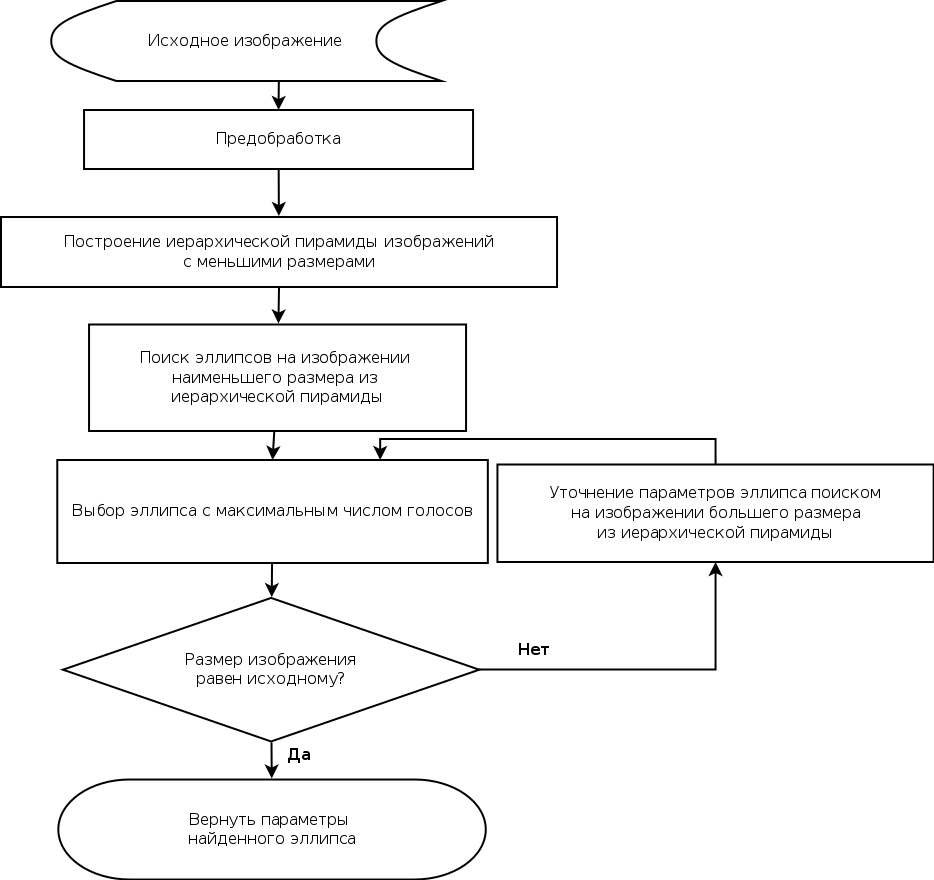
\includegraphics[width=0.9\textwidth]{img/oneellipse.png}
\end{figure}
\subsection{Подготовка изображения}
Проводится выделение краев (использовался алгоритм Кэнни). Важно отметить, что алгоритм, описанный далее, будет работать тем лучше, чем меньше на изображении шума и ненулевых пикселов,
не принадлежащих искомым эллипсам. От этого зависит как скорость работы, так и точность определения. 
По этой причине очень важно на этапе предобработки отсеять как можно больше информации, не относящейся к эллипсам. Для этих целей можно использовать размывание.
\subsection{Создание иерархической пирамиды}
Создаются уменьшенные копии изображения с выделенными краями следующим образом:
\begin{enumerate}
  \item Изображение преобразуется к квадратному $N \times N$, где $N = 2^t$, то есть является некоторой степенью двойки.
  \item Изображение переводится в матрицу со значениями 0-1, где 0 означает, что пиксел на этой позиции не является краевым, 1 - что является.

\begin{ListingEnv}[H]
\begin{lstlisting}
pyramid[0] = vector<vector<short> >(max_size,vector<short>(max_size,0)); //creating the first image (original size)
for (int i = 0; i < max_size; ++i) {
    for (int j = 0; j < max_size; ++j) {
        uchar p = resized.at<uchar>(i,j);
        if (p > 0)
            pyramid[0][i][j] = 1;
    }
}
\end{lstlisting}
\caption{Создание первого уровня иерархической пирамиды}
\label{list:level0}
\end{ListingEnv}
\item Итеративно вычисляются матрицы меньших размеров: $N$ уменьшается в два раза, после чего вычисляется новая матрица. 
При этом значение каждой ячейки вычисляется как сумма значений четырёх соответствующих ячеек матрицы, полученной на предыдущем этапе.

\begin{ListingEnv}[H]
\begin{lstlisting}
for (int i = 1; i < steps; i++)
{
    sz /= 2;
    pyramid[i] = vector<vector<short> >(sz,vector<short>(sz,0));
    for (int j = 0; j < sz; j++)
    {
        for (int k = 0; k < sz; ++k) {
            pyramid[i][j][k] = pyramid[i-1][j*2][k*2] + pyramid[i-1][j*2+1][k*2] + pyramid[i-1][j*2][k*2+1] + pyramid[i-1][j*2+1][k*2+1];
        }
    }
}
\end{lstlisting}
\caption{Создание следующих уровней иерархической пирамиды}
\label{list:otherlevels}
\end{ListingEnv}

\end{enumerate}

Процесс продолжается до тех пор, пока не будет достигнуто минимальное разрешение, заданное заранее. Большее разрешение дает большую точность, но увеличивает затраты времени, памяти и влияние шума.

\subsection{Первичный поиск}
Первичный поиск проводится модифицированным по памяти алгоритмом Хафа для матрицы минимального размера.
Модификация по памяти заключается в том, что вместо трехмерного аккумуляторного массива используется одномерный.
Этого можно добиться, используя соотношения между различными параметрами эллипса~\autocite{OneDim}.

Двойным циклом по всем парам точек контуров, найденных на изображении, выбираются и фиксируются две точки \((x_1, y_1)\) и \((x_2, y_2)\) в предположении, что они являются краевыми точками большой оси эллипса.

\begin{lstlisting}
if (((y2 == y1) && (x2 <= x1)) || (data[y2][x2] == 0)) //already been selected OR not a boundary point
    continue;
\end{lstlisting}

На этом этапе вычисляются параметры эллипса по следующим формулам:
$$x_0 = \frac{x_1 + x_2}{2}$$
$$y_0 = \frac{y_1 + y_2}{2}$$
$$a = \frac{\sqrt{(x_2 - x_1)^2 + (y_2 - y_1)^2}}{2}$$
$$\theta = \arctan(\frac{y_2 - y_1}{x_2 - x_1}).$$
Здесь \(a\) - большая полуось предпологаемого эллипса, \((x_0, y_0)\) - его центр, а \(\theta\) - поворот относительно оси \(Ox\).

\begin{ListingEnv}[H]
\begin{lstlisting}
pair<int, int> center = compute_center(x1, y1, x2, y2); //get the center point of the ellipse
int x0 = center.first;
int y0 = center.second;

double a_sq = major_axis_length_sq(x1, y1, x2, y2);
double a = sqrt(a_sq); //half of the major axis
double orient = orientation(x1, y1, x2, y2); //rotation of the ellipse
\end{lstlisting}
\caption{Вычисление параметров эллипса, шаг 1}
\label{list:majoraxis}
\end{ListingEnv}

Затем циклом по всем точкам контуров перебираются все точки \((x,y)\), которые могут принадлежать эллипсу - то есть, лежат не слишком близко к оси (не меньше заранее заданного параметра \(min\_dist\)), 
что исключает ошибочное определение прямой, как эллипса, и не дальше длины большой полуоси от центра.

\begin{lstlisting}
double d = sqrt(distance_square(x, y, x0, y0));
if ((d < min_dist) || (d > a))
    continue;
\end{lstlisting}

Для всех таких точек вычисляется длина малой полуоси \(b\) из следующего равенста:
$$b^2 = \frac{a^2d^2\sin^2\tau}{a^2-d^2\cos^2\tau}$$
Здесь \(\tau\) - угол между большой полуосью и отрезком, соединяющим центр эллипса \((x_0, y_0)\) с точкой \((x, y)\). Он определяется равенством
$$\cos\tau = \frac{a^2 + d^2 - f^2}{2ad}.$$
В аккумуляторном массиве значение, соответствующее этой длине, увеличивается.
\begin{ListingEnv}[H]
\begin{lstlisting}
double f_sq = min(distance_square(x, y, x1, y1),
               distance_square(x, y, x2, y2)); //distance to the nearest side point
double costau = (a_sq + d_sq - f_sq) / (2 * a * d);
double costau_sq = costau * costau;
double sintau_sq = 1 - costau_sq;
double b_sq = (a_sq * d_sq * sintau_sq) / (a_sq - d_sq * costau_sq);
int b = cvRound(sqrt(b_sq));
if (b > min_dist) { //voting
    acc[b] += data[y][x];
}
\end{lstlisting}
\caption{Вычисление параметров эллипса, шаг 2}
\label{list:minoraxis}
\end{ListingEnv}

После того, как все возможные точки эллипса были обработаны, в аккумуляторном массиве находится максимальный элемент. 
Значение длины малой полуоси, соответствующее ему, заносится вместе с остальными параметрами эллипса и количеством полученных голосов в список кандидатов.

После обработки всех возможных пар краевых точек из списка эллипсов-кандидатов выбирается один, имеющий наибольшее количество голосов - он и считается найденным эллипсом.

\subsection{Уточнение}
Уточнение параметров эллипса проходит итеративно с постепенным увеличением разрешения.
На каждом этапе проводится поиск, схожий с первичным, но области, в которых идет перебор возможных краевых точек, ограничен.
Если \((x, y)\) - координаты первой краевой точки эллипса, найденного на предыдущем шаге, то поиск новой точки следует 
проводить в квадрате \((2x - 1, 2y - 1), (2x + 1, 2y - 1), (2x + 1, 2y + 1), (2x - 1, 2y + 1)\). В остальном алгоритм остается тем же, что и для первичного поиска.

\subsection{Поиск нескольких эллипсов}

Если на изображении представлено несколько эллипсов, то последовательными применениями описанного выше алгоритма можно найти их все. 
Для этого после определения очередного эллипса нужно в изображении с выделенными краями обнулить все точки, принадлежащие эллипсу, после чего запустить алгоритм снова.

\begin{ListingEnv}[H]
\begin{lstlisting}
for (int i = 0; i < number_of_ellipses; i++)
{
    ellipse_data elp = ellipse_detection(edges, minimized_size, 5, 9);
    ellipses[i] = elp;
    clear_picture(edges, elp);
}
return ellipses;
\end{lstlisting}
\caption{Поиск нескольких эллипсов}
\label{list:several_ellipses}
\end{ListingEnv}

\section{Анализ алгоритма}
\subsection{Затраты по времени и памяти}
Иерархическая пирамида для входного изображения размера $N \times N$ будет иметь высоту \(log(N) - log(M) + 1\), где \(M \times M\) - размер матрицы, стоящей в её вершине. 
При этом каждый уровень имеет размер в 4 раза меньше предыдущего. Размер такой структуры данных будет составлять \(N^2 + \frac{N^2}{4} + \frac{N^2}{16} + ... < 2 * N^2\).
Такое же соотношение задаёт и количество операций, требуемых на её заполнение. В работе~\autocite{Chien} приводится оценка \(\Theta(N^2)\) для этого шага.

Затраты по времени на первичный поиск зависят от количества ненулевых пикселов на уменьшенном изображении с выделенными краями - именно по ним проводится поиск.
Пусть это количество равно \(k_0\). Тогда сложность первичного поиска составит \(({k_0}^3)\). 
Необходимо заметить, что \(k_0\), в свою очередь, зависит от минимального разрешения, которое задаётся заранее. Пусть оно составляет $M \times M$.
Тогда полученная оценка будет ограничена \(O(M^6)\). Напомним, что это разрешение не зависит от исхдных данных и является константным значением. 
Так, в программной реализации, представленной в этой работе, оно составляет \(128 \times 128\).

Количество итераций уточнения зависит от размера изображения и минимального разрешения. Пусть размер входного изображения - \(N x N\), минимальное разрешение - \(M x M\).
В этом случае понадобится \(\log(N) - \log(M)\) итераций.

Уточнение краевых точек \((x_1,y_1)\) и \((x_2,y_2)\) занимает константное время, так как проверить необходимо только точки, соответствующие найденным на предыдущем этапе.
Внутренний цикл, проходящий по всем ненулевым точкам, однако, нужно проводить полностью. 
Таким образом, оценка для каждого шага составляет \(O(k_i)\), где \(k_i\) - количество ненулевых пикселов на изображении с выделенными краями, занимающем уровень \(i\) в иерархической пирамиде.

Общая оценка для поиска эллипса составляет \(\Theta(N^2) + \displaystyle O({k_0}^3) + \sum O(k_i) \)

\section{Результаты}
В процессе работы была создана программная реализация на языке C++ (использовался компилятор g++ версии 4.9.2). 
Для загрузки изображения, сохранения результатов, а также первичной обработки (выделения границ) использовалась библиотека OpenCV версии 3.0.

Для оценки работы программы использовались как синтетические, так и реальные изображения размеров $256\times256$, $512\times512$, $1024\times1024$ с различным количеством объектов для поиска и разной степенью зашумления.
Некоторые результаты работы программы приведены в таблице~\ref{tab:results}.

\begin{table}[H]
\centering
\caption{\label{tab:results}Некоторые результаты}
\begin{tabular}{ cc }
\toprule
  Исходное изображение & Результат \\
\midrule
  \fbox{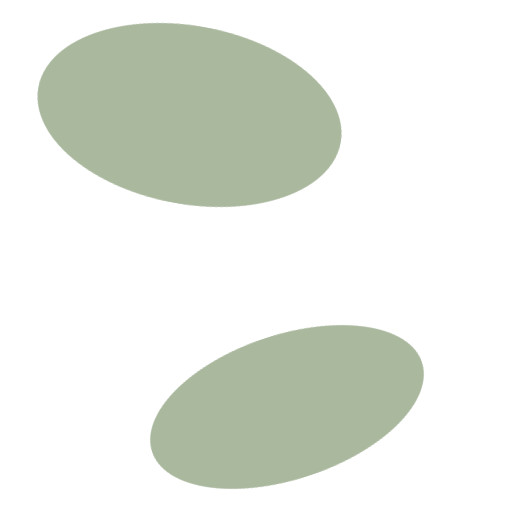
\includegraphics[width=0.25\textwidth]{img/s20.jpg}} & \fbox{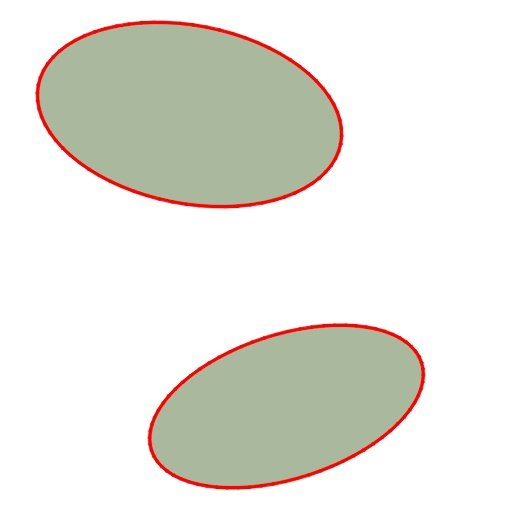
\includegraphics[width=0.25\textwidth]{img/s20r.jpg}} \\
  \fbox{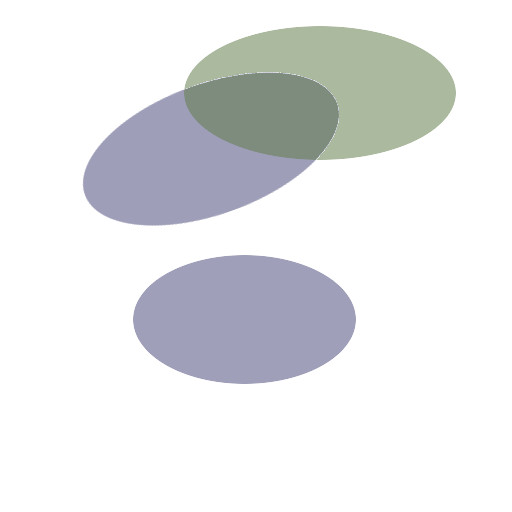
\includegraphics[width=0.25\textwidth]{img/s18.jpg}} & \fbox{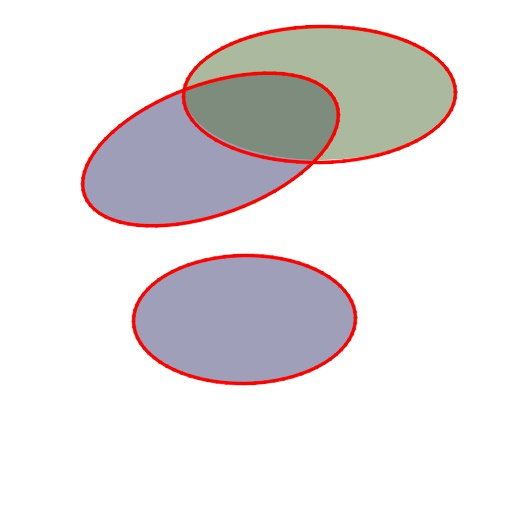
\includegraphics[width=0.25\textwidth]{img/s18r.jpg}} \\
  \fbox{
\includegraphics[width=0.25\textwidth]{img/s29.jpg}} & \fbox{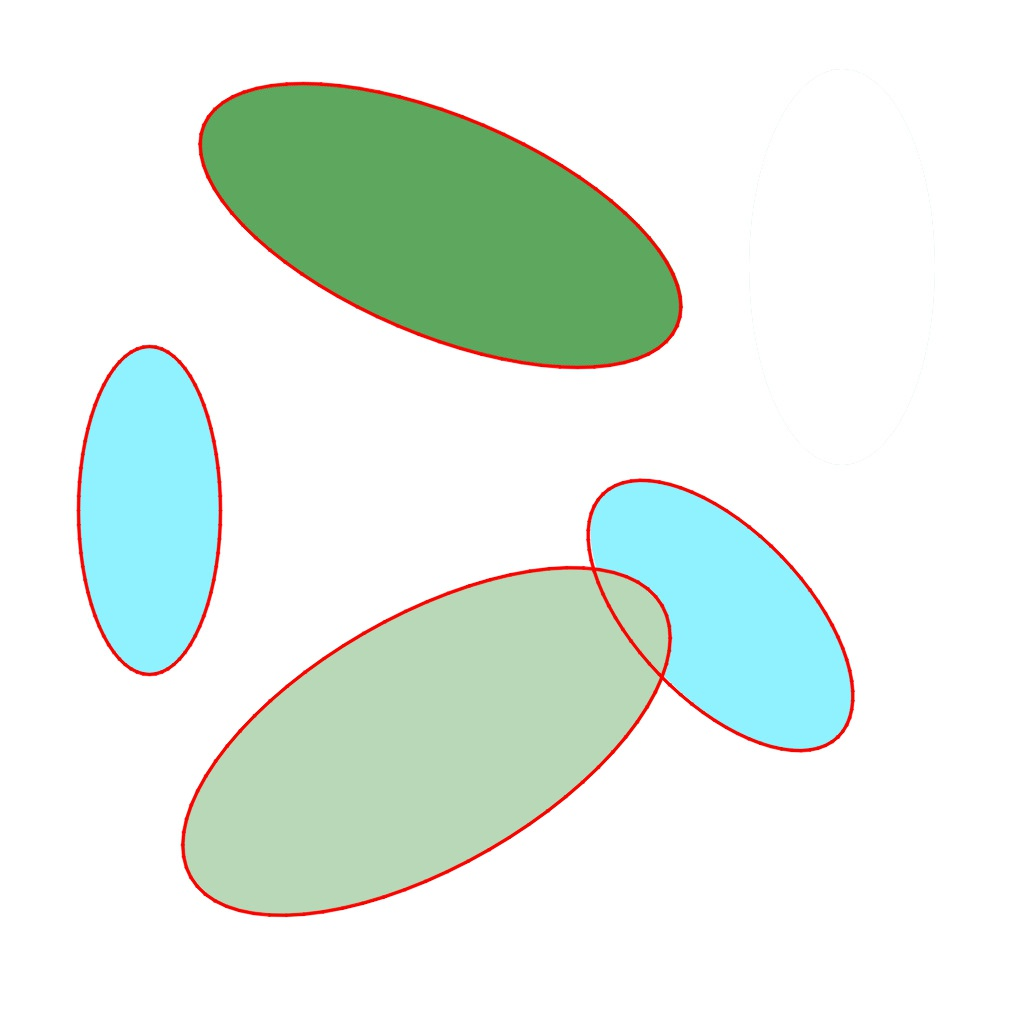
\includegraphics[width=0.25\textwidth]{img/s29r.jpg}} \\
\bottomrule
\end{tabular}
\end{table}

Гистограмма~\ref{fig:gr1} показывает зависимость между количеством не принадлежащих эллипсу точек контура и временем работы различных этапов алгоритма.
Легко заметить, что наиболее затратным по времени является первичный поиск, причем он выполняется заметно медленнее с увеличением количества обрабатываемых точек.

\small
\begin{figure}
\begin{tikzpicture}
\begin{axis}[
    ybar,
    width = 250pt,
    xlabel = {Отношение сигнал/шум},
    ylabel = {Время (сек)},
    minor tick num = 2,
    /pgf/number format/1000 sep={},
    legend style={
        at={(0.5,-0.45)},
        anchor=south,
        legend columns=-1
    }
]
\addplot coordinates {
    (0, 0.02) (0.38, 0.02) (1.15,0.02)  
};
\addplot coordinates {
    (0, 3.5) (0.38, 6.33) (1.15,18.38)
};
\addplot coordinates {
    (0, 0.27) (0.38, 0.34) (1.15,0.36)
};
\legend{Создание иерархической пирамиды, Первичный поиск, Уточнение}
\end{axis}
\end{tikzpicture}
\caption{\label{fig:gr1}Время выполнения различчных этапов алгоритма в зависимости от степени зашумлённости}
\end{figure}
\normalsize

\Conc
В результате работы был разработан алгоритм поиска эллипсов на изображении, объединивший в себе две идеи, 
позволяющие существенно сократить время работы и уменьшить объем потребляемой памяти на больших изображениях.
Разработанный алгоритм был реализован и проверен на ряде синтетических и реальных изображений. 

% Печать списка литературы (библиографии)
\printbibliography[%{}
    heading=bibintoc%
]
% Файл со списком литературы: biblio.bib
% Подробно по оформлению библиографии:
% см. документацию к пакету biblatex-gost
% http://ctan.mirrorcatalogs.com/macros/latex/exptl/biblatex-contrib/biblatex-gost/doc/biblatex-gost.pdf
% и огромное количество примеров там же:
% http://mirror.macomnet.net/pub/CTAN/macros/latex/contrib/biblatex-contrib/biblatex-gost/doc/biblatex-gost-examples.pdf

\end{document}
